% !TEX root = ../../../main.tex
% 来源：中学数学实验教材·第二册（几何）
% 章节：实验几何 / 方向、角度与平行
% 原始文件：1.tex，行 1406-1417
% 类型：tikz
% ---
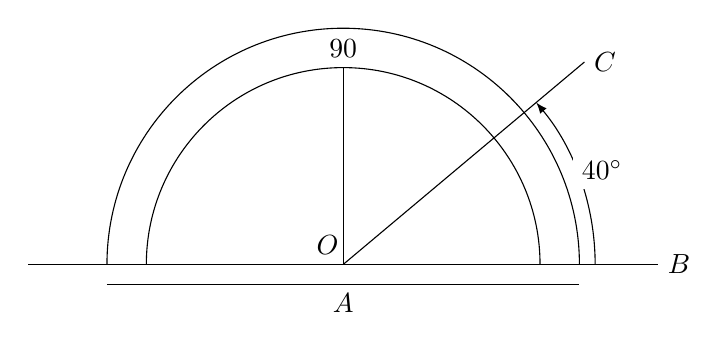
\begin{tikzpicture}[>=latex]
\draw (-4,0)--(4,0)node[right]{$B$};
\draw (2.5,0) arc (0:180:2.5);
\draw (3,0) arc (0:180:3);
\draw(0,0) --(40:4)node[right]{$C$};
\node at (-.2,0)[above]{$O$};
\draw(0,0)--(0,2.5)node[above]{$90$};
\draw[->](3.2,0) arc(0:40:3.2);
\node at (20:3.5)[fill=white]{$40^{\circ}$};
\draw(-3,-.25)--node[below]{$A$}(3,-.25);

\end{tikzpicture}	
